\section{问题三的模型建立与求解}



\subsection{多重旅行商问题}
问题三为多旅行商问题即mTSP(Multiple Traveling Salesman Problem), 与TSP类似, 该类问题同属于NPC问题. 文献\cite{surveymtsp}中对此问题进行了详细的分析, 多重旅行商问题为TSP的衍生问题, 其也可以分为多个变种, 比如根据仓库depots点的个数或者旅行商数量而区分\cite{mtsp-genetic}, 通过进化算法求解mTSP比较常见\cite{AdlemanTSP,mtsp-genetic}, 本文我们通过SOM模型对其进行求解.



\subsection{SOM模型求解多重旅行商问题}

我们将SOM模型推广, 构建了可以解决m个旅行商下n个仓库点的问题的模型som-mTSP\footnote{som-mTSP代码见支撑材料或\url{https://github.com/xdr940/som-mTSP}}. 在本文中, 考虑一个仓库点,4个旅行商的问题. 找到四条环路$G_A, G_B,G_C,G_D$, 使得四条环路的总距离最小$\sum\limits_k l_k$, 且有$A \cap B \cap C \cap D = {p_0}$, 这里$A,B,C,D$分别为四条路径的点集合.

\noindent{\textbf{问题初始化}}\\

在问题2的模型建立中, 我们参考文献\cite{isom2008}初始化神经元环形状,并迭代. 本问题中为四个旅行商的mTSP, 则需要四个神经元环, 我们这里定义为$R_A,R_B,R_C,R_D$. 同问题一(Sec.\ref{sec:method1})一样, 神经元环对应的权值向量对应着2维空间坐标, 可视化如图\ref{fig:init-mtsp}
\begin{figure}[h]
    \begin{center}
        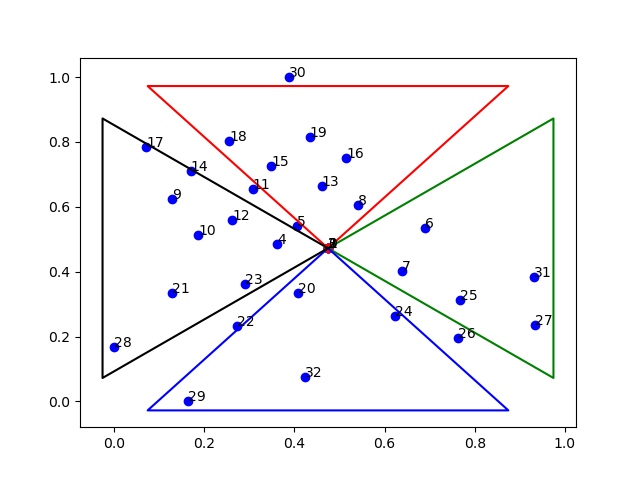
\includegraphics[width=0.55\linewidth]{fig/init2}
    \end{center}
    \caption{\textbf{som-mTSP模型中四条神经环初始化.} 在求解过程中,点的坐标已经被归一化 }
        \label{fig:init2}
  \end{figure}

\noindent{\textbf{优胜选择(Winner selection)}}\\

由于神经环在本问题中有多个, 故将优胜选择函数重新构建, 设计为两个, 一个求解对于$X_i$结点最近的神经环索引, 另一个求解在此神经环中最近神经元的索引.
\begin{eqnarray}
    k = \mathop{argmin}\limits_{k}\{ |X_i-W^k_j(n)|\beta(k) \}\\
   \nonumber
    j = \mathop{argmin}\limits_{j}\{ |X_i-W^k_j(n)|\beta(k) \} \\
    \nonumber
    \beta(k) = 1+\frac{l_k - l_{avg}}{l_{avg}},~~ k \in \{A,B,C,D\}
\end{eqnarray}

其中$l_k$是充电车在环路$G_k$行进一圈的距离,$l_{avg}$是充电车行进的平均距离, $|\cdot|$表示欧几里得距离. 此函数包括两个部分:$R_k$上的节点$W^k_j$与城市节点$X_i$之间的欧式距离,以及四个环路各自距离与平均距离的偏差$\beta(k)$. 在考虑$G_k$时,如果$l_k \leq l_{avg}$,则$R_k$上的节点的电位小于相应的欧几里得距离;因此, 将选择环$R_k$上的节点并移向所显示城市的机会更高 否则,如果$l_k \geq l_{avg}$,则选择环$R_k$上的节点的机会将减少, 该偏差可被视为需要调整每个环以获得相似距离的 minmax 约束\cite{som-mtsp2}.


\noindent{\textbf{近邻计算}}\\

我们对多个神经元环使用统一的学习率$\alpha$和半径衰减函数$\sigma$, 这里函数设定同章节(Sec.\ref{sec:preliminary})一致.

\begin{eqnarray}
    \quad & T(j,i,n) = e^{ - \frac{S^2(i,j)}{2\sigma^2(n)}}&\\
    \quad &\sigma(n) = \sigma_0e^{- n\verb|/|\tau}&
  \end{eqnarray}

\noindent{\textbf{适应(Adaption)}}\\

对于每个神经环$R_k$, 都有相同的权值更新函数:
\begin{eqnarray}
    \quad &W_j^k(n+1) =  W_j^k(n)+\alpha(n) T \cdot |X_i - W_j^k(n)|, k \in{A,B,C,D}&\\
    \nonumber
    \quad & \alpha(n) = \alpha_0e^{- n  \verb|/| \tau}&
\end{eqnarray}
这里$\alpha_0$为初始化学习率, $\tau$为衰减率, 一般设为0.99
\subsection{求解路径}
我们通过建立的som-mTSP模型, 对问题进行求解. 并预设神经元个数为每个环100个, 迭代5000次, 没100次对模型进行一次评估, 评估指标为四条环路的总长度, 并将每次最好的结果保存.

som-mTSP模型求解时间在Intel I7 8700K上共计5.6s, 求解过程以及结果可视化\footnote{支撑材料中有gif动图}见图\ref{fig:mtsp-solution}. 我们改进的模型可求解m个旅行商,n个仓库点的情况,对于问题3中$m=4, n=1$的条件, 我们将数据预处理,添加三个与$p_0$坐标相同的点, 定义为$p_1,p_2,p_3$\footnote{后文中所有点包括图示的应该减3}.
最终, 模型在迭代2200次时找到最优解,四条路径分别是:
\begin{eqnarray}
    \nonumber
    p_0 \rightarrow p_5 \rightarrow p_{13} \rightarrow p_{16} \rightarrow p_{27} \rightarrow p_{15} \rightarrow p_{12} \rightarrow p_{10}\\
    \nonumber
    p_0 \rightarrow p_{4} \rightarrow p_{21} \rightarrow p_{22} \rightarrow p_{23} \rightarrow p_{24} \rightarrow p_{28} \rightarrow p_{3}\\
    \nonumber
    p_{0} \rightarrow p_{20} \rightarrow p_{18} \rightarrow p_{25} \rightarrow p_{26} \rightarrow p_{29} \rightarrow p_{19} \rightarrow p_{17}\\
    \nonumber
    p_{0}\rightarrow p_{1}\rightarrow p_{9}  \rightarrow p_{7} \rightarrow p_{6} \rightarrow p_{14} \rightarrow p_{11} \rightarrow p_{8} \rightarrow p_{2}
\end{eqnarray}
距离分别为
\begin{eqnarray}
    \nonumber
    &l_A=0.0317137,~~l_B=0.0355413,~~l_C=0.0408157,~~l_D=0.028521&\\
    &l = l_A+l_B+l_C+l_D = 0.136592&
\end{eqnarray}

%并添加约束, 即每个神经环$R_k$求解出的环路$G_k$必须包含一个仓库点.. 

\begin{figure}[h]
    \begin{center}
        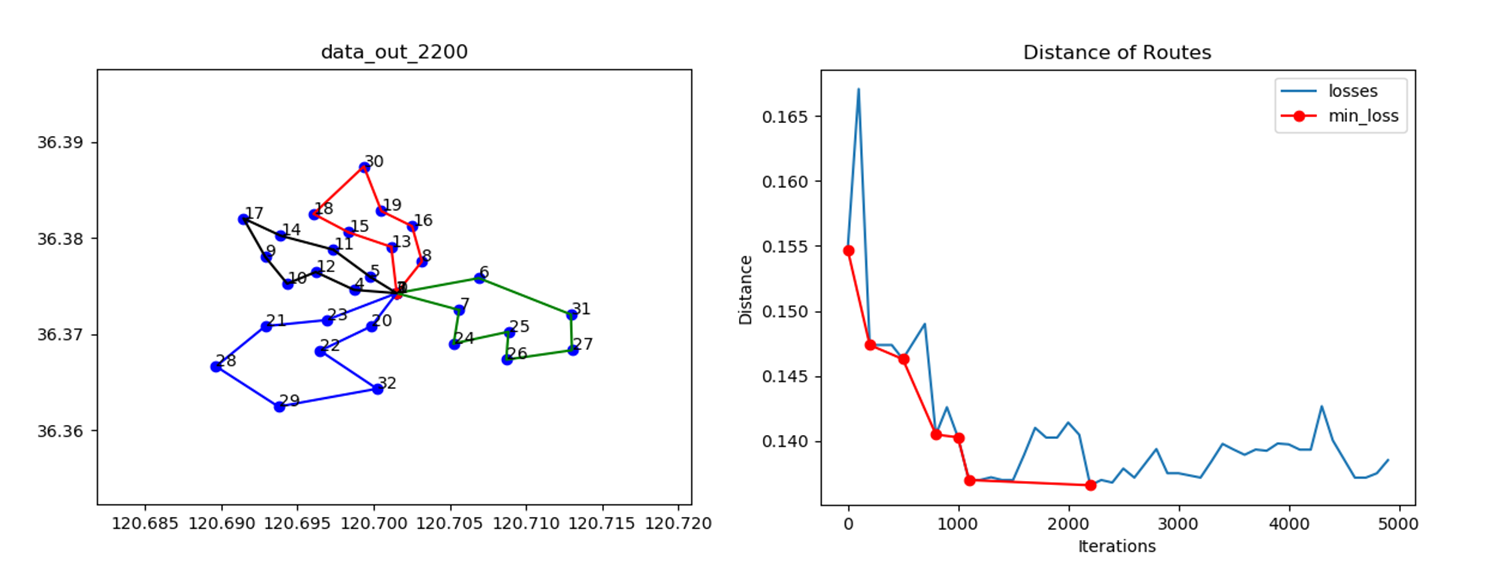
\includegraphics[width=0.95\linewidth]{fig/solution2}
    \end{center}
    \caption{\textbf{som-mTSP最优解路径.} }
        \label{fig:mtsp-solution}
  \end{figure}


\begin{figure}[h]
    \begin{center}
        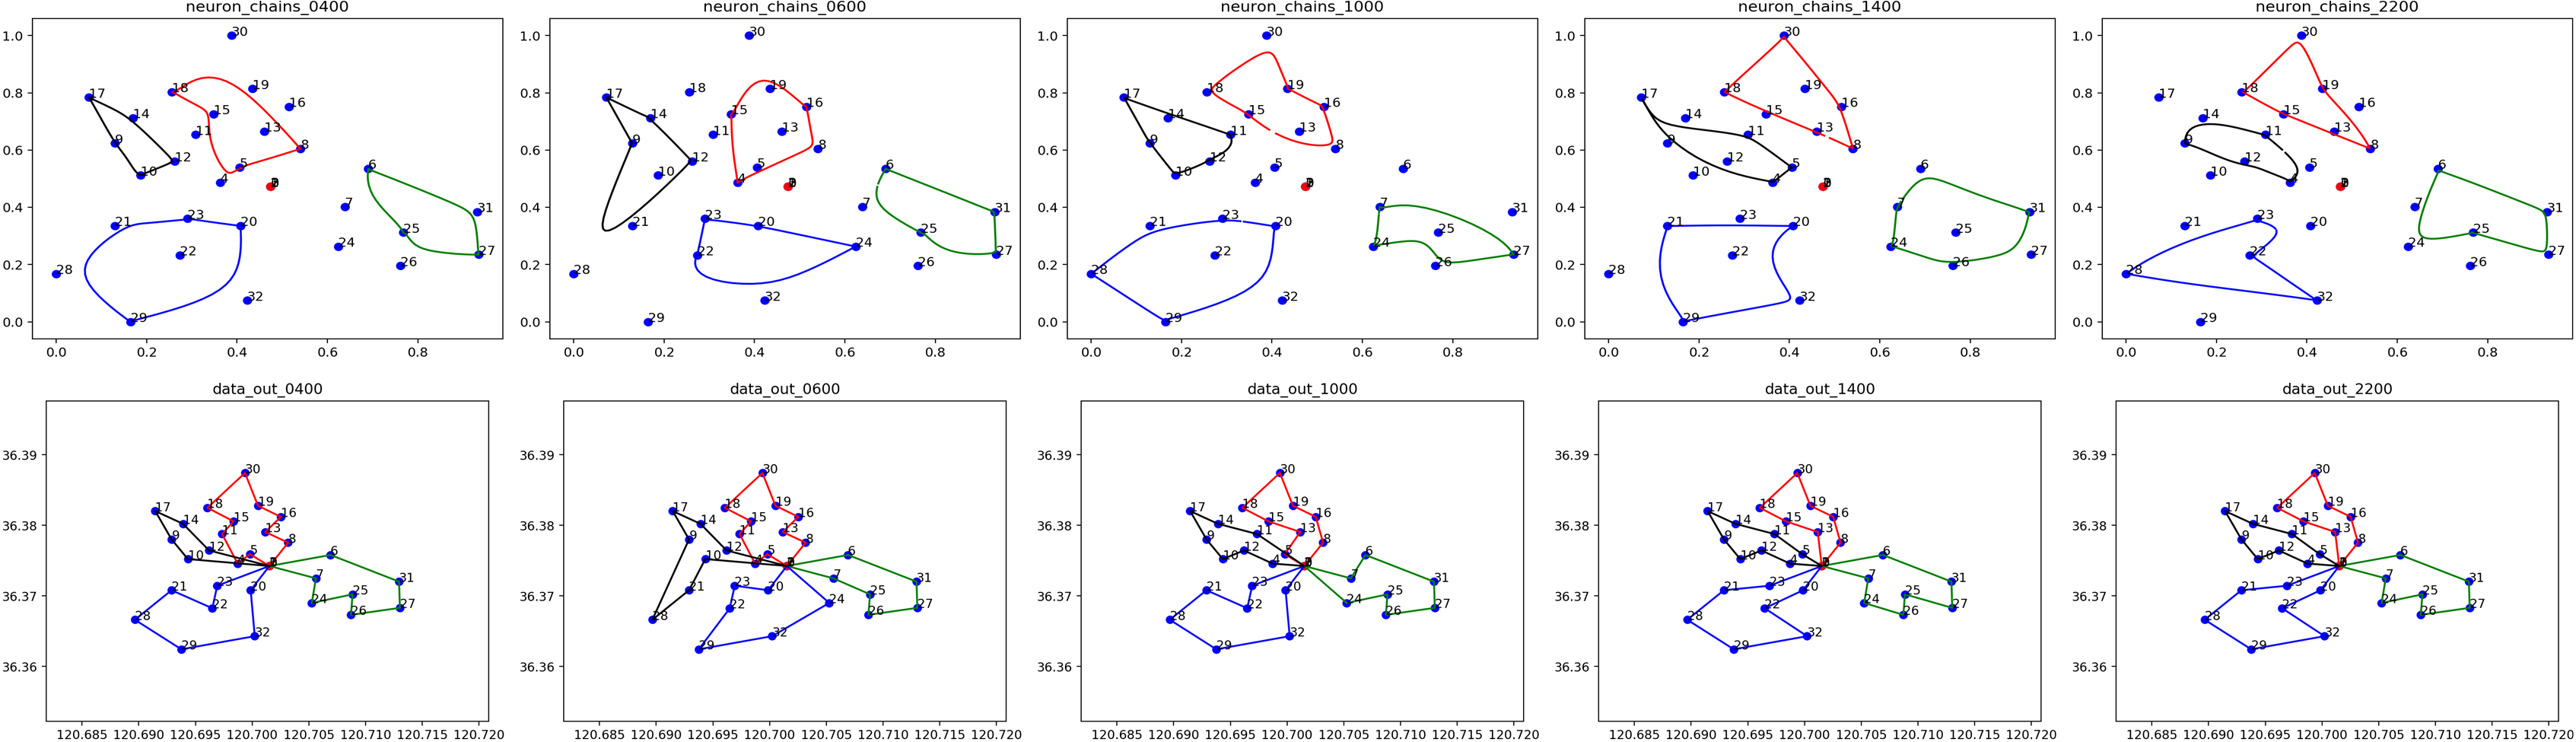
\includegraphics[width=1.0\linewidth]{fig/iteration2}
    \end{center}
    \caption{\textbf{som-mTSP求解过程.}第一行为神经元环可视化, 第二行为神经环对应的解} 
        \label{fig:iteration}
  \end{figure}

\subsection{多移动充电器下的电池最小容量求解}

在四条路径已经规划出的前提下, 每条子路径中电池最小容量与问题2求解类似(Sec.\ref{sec:method2}), 故我们使用问题二中的优化模型对本问题进行求解. 通过最小充电时间模型我们求出每个结点允许的最小充电时间, 通过最小充电时间可以求得每个子环路的最小电池容量, 而整个系统的最小电池容量即为四条环路中允许电池容量的最大值.
假设四条路径包含的点集分别为$A,B,C,D$, 则有:


\begin{eqnarray}
    c^k_{min} =r \| (\textbf{I}_k- \textbf{1}^T\textbf{a}^k )^{-1}\textbf{a}^k \frac{l^k}{v}\|_{\infty} +f ,~~k \in \{A,B,C,D\}
\end{eqnarray}
这里$\textbf{a} = [a_1, a_2, \dots a_n],~ a_i = \frac{w_i}{r+w_i}$, 且$l^k$根据som-mTSP模型已经以分别求出, 故整个系统的电池最小容量为:
\begin{eqnarray}
    c_{min} = \mathop{Max}\{c^A,c^B, c^C,c^D\}
\end{eqnarray}
